\documentclass{article}
\usepackage{graphicx}
\usepackage{subcaption}
\usepackage{amsmath}
\usepackage{amssymb}
\usepackage{pgfplots}
\pgfplotsset{compat=1.18}
\usepackage[margin=25truemm]{geometry}
\usepackage{hyperref}

\title{CSCI2750 Homework 2}
\author{Wong Cheuk Yin 1155192671}
\date{\today}

\begin{document}
    \maketitle
    \section{Problem 1}
    \subsection{Part a}

    In $\mathbb{R}^2$, take the instance $p = (1, 0)$ and the dataset
    \[
        x^{(1)} = (1, 1), \qquad x^{(2)} = (3, 0).
    \]

    \noindent Consider $x^\star$.
    \begin{itemize}
        \item $d(x^{(1)}, p) = \|x^{(1)} - p\|_2 = \|(0, 1)\|_2 = 1$.
        \item $d(x^{(2)}, p) = \|x^{(2)} - p\|_2 = \|(2, 0)\|_2 = 2$.
    \end{itemize}
    So $d(x^{(1)}, p) < d(x^{(2)}, p)$, hence $x^\star = x^{(1)}$.

    \bigskip
    \noindent Consider $x^\dagger$.

    \medskip
    \noindent The angle $g(a,b) = \arccos\bigl(\frac{a^\top b}{\|a\|_2\|b\|_2}\bigr)$ is minimized when the vectors are most aligned (smallest angle), trivial to see.
    \begin{itemize}
        \item $x^{(2)}$ and $p$ are both on the positive $x$-axis, so $g(x^{(2)}, p) = \arccos(1) = 0$.
        \item $x^{(1)}$ makes angle $\theta = 45^\circ$ with $p$, trivial to see.
    \end{itemize}
    So $g(x^{(2)}, p) < g(x^{(1)}, p)$, hence $x^\dagger = x^{(2)}$.

    \bigskip
    \noindent Thus $x^\star = x^{(1)} \neq x^{(2)} = x^\dagger$.

    \bigskip
    \noindent Geometric illustration: 
    \medskip
    \begin{center}
    \begin{tikzpicture}[scale=2.5, every node/.style={font=\small}]
        \draw[->] (-0.5,0) -- (3.5,0) node[right] {$x_1$};
        \draw[->] (0,-0.5) -- (0,1.5) node[above] {$x_2$};
        \draw[thick,->] (0,0) -- (1,0) node[below=2pt] {$p$};
        \fill (1,0) circle (1pt);
        \draw[thick,blue,->] (0,0) -- (1,1) node[above left] {$x^{(1)} = x^\star$};
        \fill[blue] (1,1) circle (1pt);
        \draw[thick,red,->] (0,0) -- (3,0) node[below=2pt] {$x^{(2)} = x^\dagger$};
        \fill[red] (3,0) circle (1pt);
        \draw (0.5,0) arc (0:45:0.5) node[midway,right=2pt] {$\theta = 45^\circ$};
        \draw[dashed] (1,0) -- (1,1) node[midway,right] {$\|x^{(1)}\!-\!p\| = 1$};
    \end{tikzpicture}
    \end{center}

    \newpage
    \subsection{Part (b)}

    For $\|p\|_2 = \|x^{(i)}\|_2 = 1$ for all $i = 1, \ldots, m$, all possible vectors of $x^{(i)}$ lies on the unit circle with center at the origin.

    \[
        d(x, p)^2 = \|x - p\|_2^2 = \|x\|_2^2 + \|p\|_2^2 - 2\, x^\top p = 2(1 - x^\top p).
    \]
    \medskip
    \noindent So we need to maximize $x^\top p$ in order to minimize $d(x, p)$.

    \noindent For unit vectors, $g(x, p) = \arccos\bigl(\frac{x^\top p}{\|x\|_2\|p\|_2}\bigr) = \arccos(x^\top p)$.\newline
    Since $\arccos$ is a decreasing function, minimizing $g(x, p)$ is equivalent to maximizing $x^\top p$ and minimize $d(x, p)$.

    \medskip
    \noindent Therefore, with the smallest $x^*$ possible, we will also have the smallest $x^\dagger$ possible.

    \section{Problem 2}
    \subsection{Part a}
    Manhattan distance: $d_1(x, y) = \sum_{i=1}^n |x_i - y_i|$.
    \begin{itemize}
        \item Non-negativity: Manhattan distance means sum of absolute differences(each element is non-negative), so it is always non-negative.
        \item identity of indiscernibles: For $d_1(x, y) = 0$, to make this happen, all corresponding elements are the same. i.e. $x = y$.
        \item Symmetry: $d_1(x, y) = d_1(y, x)$ because for absolute value, $|a - b| = |b - a|$.
        \item Triangle inequality: For each $i$, the triangle inequality for real numbers gives $|x_i - z_i| \leq |x_i - y_i| + |y_i - z_i|$. Summing over $i$:
        \[
            d_1(x, z) = \sum_{i=1}^n |x_i - z_i| \leq \sum_{i=1}^n |x_i - y_i| + \sum_{i=1}^n |y_i - z_i| = d_1(x, y) + d_1(y, z).
        \]
    
        Therefore $d_1$ is a metric.% need revise
    \end{itemize}
    \subsection{Part b}

    For each $k$, convexity of $f_k$ gives
    \[
        f_k(\alpha x_1 + (1-\alpha)x_2) \leq \alpha f_k(x_1) + (1-\alpha) f_k(x_2).
    \]
    Multiply by $c_k$, Assume $c_k \geq 0$ for all $k$ to preserve the inequality:
    \[
        c_k f_k(\alpha x_1 + (1-\alpha)x_2) \leq \alpha c_k f_k(x_1) + (1-\alpha) c_k f_k(x_2).
    \]
    Sum over for $k = 1$ to $K$:
    \[
        \sum_{k=1}^K c_k f_k(\alpha x_1 + (1-\alpha)x_2) \leq \alpha \sum_{k=1}^K c_k f_k(x_1) + (1-\alpha) \sum_{k=1}^K c_k f_k(x_2).
    \]
    If we define $f(x) = \sum_{k=1}^K c_k f_k(x)$, then by definition of $f$,
    \[
        f(\alpha x_1 + (1-\alpha)x_2) \leq \alpha f(x_1) + (1-\alpha) f(x_2).
    \]
    \noindent Therefore $f$ is convex.

    \newpage
    \subsection{Part c}

    \[
        x^\top G x - 2 r^\top A x + \|r\|_2^2
        = x^\top A^\top A x - 2 r^\top A x + \|r\|_2^2
        = \|Ax - r\|_2^2.
    \]
    \medskip
    Therefore, we have:
    \medskip
    \[
        f(x) = e^{x^\top G x - 2 r^\top A x + \|r\|_2^2}
        = e^{\|Ax - r\|_2^2}.
    \]
    \medskip
    \noindent We can write $f$ as a composition of three convex functions s.t. $f = f_1(f_2(f_3(x)))$, listing from inside to outside:
    \begin{itemize}
        \item $f_3(x) = Ax - r$, with $f_3 : \mathbb{R}^n \to \mathbb{R}^n$ (affine function);
        \item $f_2(x) = \|x\|_2^2$, with $f_2 : \mathbb{R}^n \to \mathbb{R}$ (squared norm, convex);
        \item $f_1(x) = e^{x}$, with $f_1 : \mathbb{R} \to \mathbb{R}$ (strictly convex because exponential, non-decreasing).
    \end{itemize}
    \medskip
    By convex-preserving rules...
    
    \medskip
    \noindent$f_2(f_3(x)) = \|Ax - r\|_2^2$ is convex because it is the composition of a convex function with an affine function.

    \medskip
    \noindent$f_1(f_2(f_3(x))) = e^{\|Ax - r\|_2^2}$ is convex because it is the composition of a non-decreasing convex function with another convex function.
    
    \medskip
    \noindent Therefore $f$ is convex.

    \section{Problem 3}
    \subsection{Part a}

    Both terms in $f$ are non-negative and are thus minimized when $x_1 = 0$ and $x_2 = 0$, giving $f(0,0) = 0$.
    
    \medskip
    \noindent Also, The point $(0,0)$ satisfies the constraint $x_1^2 + x_2^2 \le 1$, so the solution is feasible as well.
    \[ x^\star = (0,0), \qquad f(x^\star) = 0. \]

    \subsection{Part b}

    We write (P) in the standard convex form
    \[
        \min_{x \in \mathbb{R}^2} f(x)
        \quad \text{s.t.} \quad g(x) \le 0,
    \]
    where
    \[
        f(x) = \frac{1}{4}x_1^4 + \frac{3}{2}x_2^2,
        \qquad
        g(x) = x_1^2 + x_2^2 - 1.
    \]

    \noindent $f(x)$ is convex because:
    \begin{itemize}
        \item The function $x^2$ is convex, so $x_1^2$ and $x_2^2$ are convex functions of $x_1$ and $x_2$ respectively.
        \item The function $x^4$ can be written as $x^4 = (x^2)^2$. $x^2$ is convex and non-decreasing for $x \ge 0$. For the inner $x^2$, it must be non-negative, so we can see the outer function is non-decreasing. It is a composition of a convex non-decreasing convex function with another convex function, hence $x^4$ and thus $x_1^4$ are convex.
        \item Both $x_1^4$ and $x_2^2$ is scaled by a positive constant, and sumed up to form $f(x)$. In this case, the convexity is preserved.
    \end{itemize}
    
    \newpage
    \subsection{Part c}
    \[
        \mathcal{L}(x_1,x_2,\alpha)
        = \frac{1}{4}x_1^4 + \frac{3}{2}x_2^2
          + \alpha\,(x_1^2 + x_2^2 - 1).
    \]
    %where $\alpha \ge 0$ is the Lagrange multiplier.
    Consider the KKT conditions:
    \begin{itemize}
        \item \textbf{Stationarity:} take derivatives of $\mathcal{L}$ with respect to $x_1$ and $x_2$ and set them to zero:
        \[
            \frac{\partial \mathcal{L}}{\partial x_1}
            = x_1^3 + 2\alpha x_1 = 0 
            \quad\Rightarrow\quad x_1(x_1^2 + 2\alpha) = 0,
        \]
        \[
            \frac{\partial \mathcal{L}}{\partial x_2}
            = 3x_2 + 2\alpha x_2 = 0 
            \quad\Rightarrow\quad x_2(3 + 2\alpha) = 0.
        \]
        \item \textbf{Primal feasibility:} 
        \[
            g(x) = x_1^2 + x_2^2 - 1 \le 0.
        \]
        \item \textbf{Dual feasibility:} 
        \[
            \alpha \ge 0.
        \]
        \item \textbf{Complementary slackness:} 
        \[
            \alpha\, (x_1^2 + x_2^2 - 1) = 0.
        \]
    \end{itemize}

    \noindent For $\alpha \ge 0$, we have no solution for $x_1^2 + 2\alpha = 0$ and $3 + 2\alpha = 0$, so we must have
    \[
        x_1 = 0, \quad x_2 = 0.
    \]
    \noindent Then Complementary slackness gives $\alpha(x_1^2 + x_2^2 - 1) = 0$. Since $x_1 = 0$ and $x_2 = 0$, we have $x_1^2 + x_2^2 - 1 = -1 < 0$, forcing $\alpha = 0$.
    
    \medskip
    \noindent Thus the KKT point is $(x_1^\star, x_2^\star, \alpha^\star) = (0,0,0)$, consistent with the solution found in Part (a).

    \subsection{Part d}
    In MATLAB, I used the following code to solve the problem:
    \begin{verbatim}
        cvx_begin
            variables x1 x2
            minimize( 0.25 * pow_pos(x1, 4) + 1.5 * square(x2) )
            subject to
                square(x1) + square(x2) <= 1;
        cvx_end
    \end{verbatim}
    
    \noindent The result is ``Optimal value (cvx\_optval): +3.20163e-12'', essentially the same as the solution found in Part (a) with a extremely small numerical error.

    \section{Problem 4}
    \subsection{list of wikipages}
    Five modern scientists:
    \begin{itemize}
        \item Stephen Hawking: \url{https://en.wikipedia.org/wiki/Stephen_Hawking}
        \item James Watson: \url{https://en.wikipedia.org/wiki/James_Watson}
        \item Tu Youyou: \url{https://en.wikipedia.org/wiki/Tu_Youyou}
        \item Albert Einstein: \url{https://en.wikipedia.org/wiki/Albert_Einstein}
        \item Timothy Berners-Lee: \url{https://en.wikipedia.org/wiki/Timothy_Berners-Lee}
    \end{itemize}

    \noindent Five athletes:
    \begin{itemize}
        \item Kobe Bryant: \url{https://en.wikipedia.org/wiki/Kobe_Bryant}
        \item Cristiano Ronaldo: \url{https://en.wikipedia.org/wiki/Cristiano_Ronaldo}
        \item Lionel Messi: \url{https://en.wikipedia.org/wiki/Lionel_Messi}
        \item Michael Phelps: \url{https://en.wikipedia.org/wiki/Michael_Phelps}
        \item Usain Bolt: \url{https://en.wikipedia.org/wiki/Usain_Bolt}
    \end{itemize}
    
    \noindent all pages are accessed on 2026-02-20. 12:00nn.
    \subsection{Dictionary}
    I chose the following words as the dictionary:
    \begin{itemize}
        \item Technology
        \item Speed
        \item Death
        \item Physics
        \item Olympic
        \item Rival
        \item Champion
    \end{itemize}
    \subsection{Word occurrence counts}
    Counts of the 7 dictionary words on each Wikipedia page:
    \medskip
    \begin{center}
    \begin{tabular}{l|ccccccc}
        \hline
        Page & Technology & Speed & Death & Physics & Olympic & Rival & Champion \\
        \hline
        Stephen Hawking & 18 & 2 & 46 & 107 & 0 & 0 & 1 \\
        James Watson & 8 & 0 & 7 & 6 & 0 & 0 & 0 \\
        Tu Youyou & 18 & 0 & 1 & 4 & 2 & 0 & 0 \\
        Albert Einstein & 12 & 7 & 19 & 189 & 0 & 0 & 0 \\
        Timothy Berners-Lee & 34 & 0 & 0 & 3 & 1 & 0 & 0 \\
        Kobe Bryant & 1 & 1 & 62 & 0 & 38 & 1 & 6 \\
        Cristiano Ronaldo & 0 & 1 & 4 & 0 & 7 & 1 & 3 \\
        Lionel Messi & 0 & 3 & 1 & 0 & 15 & 12 & 19 \\
        Michael Phelps & 1 & 1 & 2 & 0 & 326 & 5 & 11 \\
        Usain Bolt & 9 & 24 & 0 & 3 & 177 & 8 & 26 \\
        \hline
        \textbf{Total} & 101 & 39 & 142 & 312 & 566 & 27 & 66 \\
        \hline
    \end{tabular}
    \end{center}

    \newpage
    \subsection{Heatmap}
    By using  MATLAB, I generated the following heatmap:
    \begin{figure}[h]
        \centering
        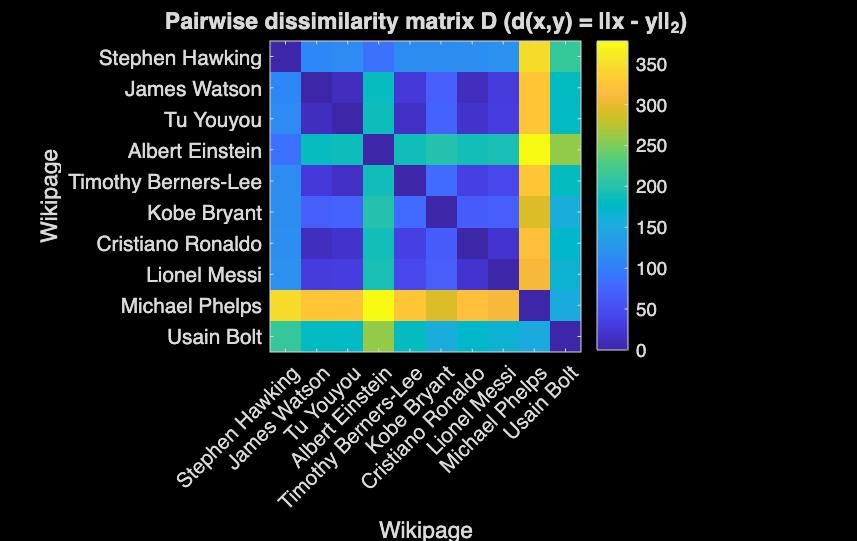
\includegraphics[width=0.8\textwidth]{heatmap.png}
        \caption{Heatmap of the word occurrence counts}
    \end{figure}

    \subsection{Brief analyis}

    We can make use of the euclidean distance of count vector to measure the similarity between two pages.\newline
    The smaller the distance, the more similar the two pages are.\newline
    There for we can group the pages into different clusters based on the distance.\newline
    A heatmap is a good way to visualize the similarity between two pages.

    \newpage
    \subsection{Appendix}
    Below is the MATLAB code used to generate the heatmap:
    \begin{verbatim}
        % Word-count vectors
        X = [18  2 46 107   0   0  1;   % Stephen Hawking
        8  0  7   6   0   0  0;   % James Watson
        18  0  1   4   2   0  0;   % Tu Youyou
        12  7 19 189   0   0  0;   % Albert Einstein
        34  0  0   3   1   0  0;   % Timothy Berners-Lee
        1  1 62   0  38   1  6;   % Kobe Bryant
        0  1  4   0   7   1  3;   % Cristiano Ronaldo
        0  3  1   0  15  12 19;   % Lionel Messi
        1  1  2   0 326   5 11;   % Michael Phelps
        9 24  0   3 177   8 26];  % Usain Bolt

        names = {'Stephen Hawking', 'James Watson', 'Tu Youyou', 'Albert Einstein', ...
                 'Timothy Berners-Lee', 'Kobe Bryant', 'Cristiano Ronaldo', ...
                 'Lionel Messi', 'Michael Phelps', 'Usain Bolt'};
        n = size(X, 1);
        D = zeros(n, n);
        for i = 1:n
            for j = 1:n
                diff = X(i,:) - X(j,:);
                D(i,j) = sqrt(sum(diff.^2));
            end
        end

        % Heatmap
        figure;
        imagesc(D);
        colorbar;
        title('Pairwise dissimilarity matrix D (d(x,y) = ||x - y||_2)');
        xlabel('Wikipage');
        ylabel('Wikipage');
        set(gca, 'XTick', 1:n, 'XTickLabel', names, 'XTickLabelRotation', 45);
        set(gca, 'YTick', 1:n, 'YTickLabel', names);
        axis square;

        saveas(gcf, 'heatmap.png');
    \end{verbatim}

\end{document}